%MCQMC, April 6-11, 2014
%Requires graphics files
%  sob256pts.eps, scrsob256pts.eps, PlotFWTCoefUse256.eps KeistercubSobolErrTime.eps

%%%%%%%%%%%%%%%% Springer %%%%%%%%%%%%%%%%%%%%%%%%%%%%%%%%%%
\documentclass[graybox,footinfo]{svmult}

\smartqed
\usepackage{mathptmx}       % selects Times Roman as basic font
\usepackage{helvet}         % selects Helvetica as sans-serif font
\usepackage{courier}        % selects Courier as typewriter font
\usepackage{type1cm}        % activate if the above 3 fonts are
                            % not available on your system
\usepackage{graphicx}       % standard LaTeX graphics tool
                            % when including figure files

\usepackage{array,colortbl}
\usepackage{amsmath,amsfonts,amssymb,bm} % no amsthm, Springer defines Theorem, Lemma, etc themselves
%\usepackage[mathx]{mathabx}
\DeclareFontFamily{U}{mathx}{\hyphenchar\font45}
\DeclareFontShape{U}{mathx}{m}{n}{
      <5> <6> <7> <8> <9> <10>
      <10.95> <12> <14.4> <17.28> <20.74> <24.88>
      mathx10
      }{}
\DeclareSymbolFont{mathx}{U}{mathx}{m}{n}
\DeclareFontSubstitution{U}{mathx}{m}{n}
\DeclareMathAccent{\widecheck}      {0}{mathx}{"71}

% Note that Springer defines the following already:
%
% \D upright d for differential d
% \I upright i for imaginary unit
% \E upright e for exponential function
% \tens depicts tensors as sans serif upright
% \vec depicts vectors as boldface characters instead of the arrow accent
%
% Additionally we throw in the following common used macro's:
\newcommand{\Z}{\mathbb{Z}} % integers
\newcommand{\C}{\mathbb{C}} % complex numbers
\newcommand{\R}{\mathbb{R}} % reals
\newcommand{\N}{\mathbb{N}} % natural numbers {1, 2, ...}
\newcommand{\Q}{\mathbb{Q}} % rationals
\newcommand{\F}{\mathbb{F}} % field, finite field
\newcommand{\floor}[1]{\left\lfloor #1 \right\rfloor} % floor
\newcommand{\ceil}[1]{\left\lceil #1 \right\rceil}    % ceil
\newcommand{\rd}{\,\mathrm{d}} % differential symbol for use in integrals
% vectors as boldsymbols:
\newcommand{\bszero}{\boldsymbol{0}} % vector of zeros
\newcommand{\bsone}{\boldsymbol{1}}  % vector of ones
\newcommand{\bst}{\boldsymbol{t}}    % vector t
\newcommand{\bsu}{\boldsymbol{u}}    % vector u
\newcommand{\bsv}{\boldsymbol{v}}    % vector v
\newcommand{\bsw}{\boldsymbol{w}}    % vector w
\newcommand{\bsx}{\boldsymbol{x}}    % vector x
\newcommand{\bsy}{\boldsymbol{y}}    % vector y
\newcommand{\bsz}{\boldsymbol{z}}    % vector z
\newcommand{\bsDelta}{\boldsymbol{\Delta}}    % vector \Delta
% sets as Euler fraks:
\newcommand{\setu}{\mathfrak{u}}
\newcommand{\setv}{\mathfrak{v}}
% indicator boldface 1:
\DeclareSymbolFont{bbold}{U}{bbold}{m}{n}
\DeclareSymbolFontAlphabet{\mathbbold}{bbold}
\newcommand{\ind}{\mathbbold{1}}


\usepackage{microtype} % good font tricks

\usepackage[colorlinks=true,linkcolor=black,citecolor=black,urlcolor=black]{hyperref}
\urlstyle{same}
\usepackage{bookmark}
\pdfstringdefDisableCommands{\def\and{, }}
\makeatletter % to avoid hyperref warnings:
  \providecommand*{\toclevel@author}{999}
  \providecommand*{\toclevel@title}{0}
\makeatother

%Fred's additions
%\usepackage{amsmath,datetime,xmpmulti,mathtools,bbm,array,booktabs,alltt,xspace,mathabx,tikz,pifont,graphicx}
\usepackage{mathtools,array,booktabs}
\DeclareMathOperator{\ok}{ok}

%%%%%%%%%%%%%%%%%%%%%%%%%%%%%%%%%%%%%%%%%%%%%%%%%%%%%%%%%%%%%%%%%%%%%%%%%%%%%%%%%%%%%%%%%
\begin{document}
\spnewtheorem{algo}{Algorithm}{\bf}{\rm}
\newcommand{\bsa}{\boldsymbol{a}}    %%% vector a
\newcommand{\bsh}{\boldsymbol{h}}    %%% vector h
\newcommand{\bsi}{\boldsymbol{i}}    % vector i
\newcommand{\bsj}{\boldsymbol{j}}    %%% vector j
\newcommand{\bsk}{\boldsymbol{k}}    % vector k
\newcommand{\bsl}{\boldsymbol{l}}    % vector l
\newcommand{\bsr}{\boldsymbol{r}}    % vector r
\newcommand{\bsnu}{\boldsymbol{\nu}}    % vector nu
\newcommand{\dif}{{\rm d}}			%%% Differential dx
\newcommand{\me}{\text{e}}			%%% Do not
\newcommand{\cc}{\mathcal{C}}
\newcommand{\cm}{\mathcal{M}}		%%%
\newcommand{\cl}{\mathcal{L}}
\newcommand{\cn}{\mathcal{N}}
\newcommand{\Order}{\mathcal{O}}
\newcommand{\cp}{\mathcal{P}}
\newcommand{\cx}{\mathcal{X}}
\newcommand{\natm}{\N_{0,m}}
\newcommand{\cube}{[0,1)^d}
\newcommand{\hf}{\hat{f}}
\newcommand{\rf}{\mathring{f}}
\newcommand{\tf}{\tilde{f}}
\newcommand{\hg}{\hat{g}}
\newcommand{\hI}{\hat{I}}
\newcommand{\tvk}{\tilde{\bsk}}
\newcommand{\hS}{\widehat{S}}
\newcommand{\tS}{\widetilde{S}}
\newcommand{\wcS}{\widecheck{S}}
\newcommand{\rnu}{\mathring{\nu}}
\newcommand{\tnu}{\widetilde{\nu}}
\newcommand{\hnu}{\widehat{\nu}}
\newcommand{\hbsnu}{\widehat{\bsnu}}   %%%
\newcommand{\homega}{\widehat{\omega}}
\newcommand{\wcomega}{\mathring{\omega}}
\newcommand{\fC}{\mathfrak{C}}
\newcommand{\nodes}{\{\bsz_i\}_{i=0}^{\infty}}
\newcommand{\nodesn}{\{\bsz_i\}_{i=0}^{n-1}}
\newcommand{\norm}[1]{\ensuremath{\left \lVert #1 \right \rVert}}
\newcommand{\abs}[1]{\ensuremath{\left |  #1 \right |}} %%%
\newcommand{\bigabs}[1]{\ensuremath{\bigl \lvert #1 \bigr \rvert}}
\newcommand{\Bigabs}[1]{\ensuremath{\Bigl \lvert #1 \Bigr \rvert}}
\newcommand{\biggabs}[1]{\ensuremath{\biggl \lvert #1 \biggr \rvert}}
\newcommand{\Biggabs}[1]{\ensuremath{\Biggl \lvert #1 \Biggr \rvert}}
\newcommand{\ip}[3][{}]{\ensuremath{\left \langle #2, #3 \right \rangle_{#1}}}



\title*{Adaptive Multidimensional Integration Based on Rank-1 Lattices}
\author{Fred J. Hickernell \and Llu\'is Antoni Jim\'enez Rugama}
\institute{Fred J. Hickernell \and Llu\'is Antoni
\at Department of Applied Mathematics,  Illinois Institute of Technology, 10 W. 32$^{\text{nd}}$ Street, E1-208, Chicago, IL 60616, USA
\email{hickernell@iit.edu}, \email{ljimene1@hawk.iit.edu}}
\maketitle

\abstract{}

\section{Introduction}
Quasi-Monte Carlo methods are used to approximate multidimensional integration in $\cube$ although this can be generalized in any other domain. People have traditionally used these methods, together with the Monte Carlo methods, because they do not suffer from the \textit{Curse of dimensionality}, i.e. the convergence rate does not depend on the dimension. For example, the dimension-dependent Simpson's rule has $\Order(n^{-4/d})$ and is improved when the dimension $d$ is greater than 4, by the Quasi-Monte Carlo method which has $\Order(n^{-(1-\varepsilon)})$ for small $\varepsilon$. Here $n$ represents the number of data points.

However, the convergence rate does not give us enough information about the absolute error which can be used for building an adaptive algorithm. Although a first approach could be using the Koksma-Hlawka inequality, the main practical disadvantage for it is computing the variation $V(f)$. Thus, in this paper we define a new bound on the absolute error based on the decay of the Fourier coefficients. This will 
Intuitively, a function whose Fourier coefficients decay quickly would 
We use Rank-1 Lattices...

\section{Rank-1 Integration Lattices in $\cube$}
The integrands that will be considered are periodic functions over $\cube$. One may change the domain to some more general by using transformations such as explained in.... ....

As defined in \cite{SloJoe94}, integration lattices $\cm$ are discrete groups in $\R^d$ containing $\Z^d$. Since our domain of interest is $\cube$, the points in the lattice we consider are $\cp:=\cm/\Z^d$. More concisely, the lattice $\cp_m$ with $b^m$ points is built using a generating vector $\bsh$ in $\Z^d$ where $\gcd(h_1,\dots,h_d,b^m)=1$:

\begin{equation}
\cp_m :=\left\{\bsh\frac{j}{b^m}\pmod 1\, ;\, j\in\F_{b^m}\right\}
\end{equation}

Plot example...

In the following, a structure to these points is provided.


\subsection{Group-Like Structures}
Consider $\cube$ with the additive operation $\oplus:\cube \times \cube \to \cube$, $\bsx\oplus\bsy=\bsx+\bsy\pmod 1$. Indeed, $(\cube,\oplus)$ is an Abelian group. Note that $\bszero$ is the additive identity and that the unique additive inverse of $\bsx$ is $\ominus \bsx:=\bold{1}-\bsx$, where $\bsx \ominus \bst$ means $\bsx \oplus (\ominus \bst)$. Moreover, such a set $\cube$ is also a field over $\Z$ when the multiplicative operation is seen by means of $\oplus$:

\[
a \bsx:=\underbrace{\bsx \oplus \cdots \oplus \bsx}_{a \text{ times}}\ \forall a \in \N, \qquad a \bsx:=\underbrace{\ominus\bsx \ominus \cdots \ominus \bsx}_{-a \text{ times}}\ \forall a \in \Z\setminus\N_0.
\]
 
The set $\Z^d$ is used to index Fourier series expressions for the integrands. Hence, for that application we define the bilinear operation $\ip{\cdot}{\cdot}: \Z^d \times \cube \to \cube$,
\begin{subequations} \label{bilinear}
\begin{equation}
\ip{\bsk}{\bsx}=\bsk^T\bsx\pmod 1.
\end{equation}

For all $\bst, \bsx \in \cube$, $\bsk, \bsl \in \Z^d$, and $a \in \Z$, it follows that

\begin{gather}
\ip{\bsk}{\bszero} = \ip{\bszero}{\bsx} = 0,\\
\ip{\bsk}{a \bsx \oplus \bst} = a\ip{\bsk}{\bsx} + \ip{\bsk}{\bst} \pmod 1 \label{bilinearlinxprop} \\
\ip{a \bsk + \bsl}{\bsx} = a\ip{\bsk}{\bsx} + \ip{\bsl}{\bsx} \pmod 1, \label{bilinearlinkprop}\\
\ip{\bsk}{\bsx} = 0 \ \forall \bsk \in \Z^d \ \implies \ \bsx=\bszero.\label{bilinearlinzeroprop}
\end{gather}
\end{subequations}

\subsection{Embedded Rank-1 Lattices and Dual Nets}
By construction, $\cp_m := \{\bsz_i\}_{i=0}^{b^m-1}$ doted with $\oplus$ is an Abelian group. Suppose that there exists a sequence of points in $\cube$, denoted $\cp_\infty =\{\bsz_i\}_{i=0}^{\infty}$ and closed under $\oplus$. Thus, $\{0\}=\cp_0\subseteq\dots\subseteq\cp_m\subseteq\dots\subseteq\cp_\infty$. is an embedded tower of Rank-1 Lattices.

Furthermore, $\cp_\infty$ is assumed to satisfy the following properties:

\begin{subequations} \label{cpinfvector}
\begin{gather}
\{\bsz_{1}, \bsz_{b}, \bsz_{b^2}, \ldots\} \text{ is a set of linearly independent points}, \\
b\bsz_{b^m}=\bsz_{b^{m-1}},\label{latpropb}\\
\bsz_i = \sum_{\ell=0}^{\infty} i_l \bsz_{b^\ell}, \qquad \text{where }\bsi=(i_0, i_1, i_2, \ldots ) \in \F_b^\infty, \label{latpropc}\\
\ip{\bsk}{\bsz_i} =  0 \ \forall i \in \N_0   \ \implies \ \bsk=\bszero. \label{latpropd}
\end{gather}
\end{subequations}
Note that from \eqref{bilinear} together with \eqref{latpropb} it follows,
\begin{equation}\label{assumgenip}
\ip{\bsk}{\bsz_{b^{m-1}}}=\ip{b\bsk}{\bsz_{b^m}}
\end{equation}
This property is relevant for defining a Fast Fourier Transform adapted to our Rank-1 Lattices in section \ref{...}....

One example is the extensible $Rank-1$ Lattices from \cite{HicNie03a}. In this case, the generating vector $\bsh$ can be seen in each coordinate as an infinite digit integer. In addition, for every $\cp_m$ we can choose a generator. If we want $\bst_{b^{m-1}}=\bsh\frac{j_m}{b^m}$ to the the generator of $\cp_m$, it only suffices to verify that $\gcd(j_m,b^m)=1$ with $j_m\in\F_{b^m}$. This sequence $j_0,j_1,\dots$ defines $\cp_\infty$. In addition, to satisfy equation \eqref{latpropb},  $j_m$'s: $ b^{m-1} \mid j_m-j_{m-1}\Rightarrow j_m=j_{m-1}+b^{m-1},\;\forall m\in\N$. A part from that, \eqref{latpropc} implies that the order of the elements in $\cp_\infty$ given the generators must follow the Sobol order.

The bilinear operation previously mentioned let us also define the \emph{dual Lattice} corresponding to $\cp_m$ as
\begin{align}
\nonumber
\cp^{\perp}_m &= \{\bsk \in \Z^d : \ip{\bsk}{\bsz_i} = 0, \ i=0, \ldots, b^m-1\} \\
&= \{\bsk \in \Z^d : \ip{\bsk}{\bsz_{b^{l}}} = 0, \ l=0, \ldots, m-1\}.\label{dualdef}
\end{align}
By this definition $\cp^{\perp}_{0}=\Z^d$ and the properties \eqref{bilinear} together with \eqref{cpinfvector}, imply also that $\cp^{\perp}_m$ are subgroups with
\begin{equation}\label{dualemb}
\Z^d=\cp^{\perp}_{0}\supseteq\dots\supseteq\cp^{\perp}_{m}\supseteq\dots\supseteq\cp^{\perp}_{\infty}=\{0\}.
\end{equation}

One example of Rank-1 Lattice and its dual Lattice can be found below:
\begin{figure}[h!]
\centering
\begin{tabular}{>{\centering}p{5cm}>{\centering}p{5cm}}
\includegraphics[width=5cm]{Images/sob256pts.eps} &
\includegraphics[width=5cm]{Images/scrsob256pts.eps}\tabularnewline
a) & b)
\end{tabular}
\caption{a) 256 Sobol' points, b) 256 scrambled and digitally shifted Sobol' points \label{Sobolfig}}
\end{figure}

\section{Fourier Series}

The integrands are assumed to be periodic and belong to some subset of $\cl_2(\cube)$, the space of square integrable functions. For non periodic integrands we suggest some transforms in Appendix A. The $\cl_2$ inner product is defined as
\[
\ip[2]{f}{g} = \int_{\cube} f(\bsx) \overline{g(\bsx)} \, \dif \bsx.
\]
Let $\{\varphi(\cdot,\bsk) \in \cl_2(\cube) : \bsk \in \Z^d\}$ be the complete orthonormal Fourier function \emph{basis} for $\cl_2(\cube)$, i.e.,
\[
\varphi(\bsx,\bsk)  = \me^{2 \pi \sqrt{-1} \ip{\bsk}{\bsx}}, \qquad \bsk \in \Z^d, \ \bsx \in \cube.
\]
Then any function in $\cl_2$ may be written in series form as
\begin{equation} \label{Fourierdef}
f(\bsx) = \sum_{\bsk \in \Z^d} \hf(\bsk) \varphi(\bsx,\bsk), \quad \text{where } \hf(\bsk) = \ip[2]{f}{\varphi(\cdot,\bsk)},
\end{equation}
and the inner product of two functions in $\cl_2$ is the $l_2$ inner product of their series coefficients:
\[
\ip[2]{f}{g} = \sum_{\bsk \in \Z^d} \hf(\bsk)\overline{\hg(\bsk)} =: \ip[2]{\bigl(\hf(\bsk)\bigr)_{\bsk \in \Z^d}}{\bigl ( \hg(\bsk)\bigr )_{\bsk \in \Z^d}}.
\]

Because the set $\cp_m$ is closed under $\oplus$, we can derive a useful formula for the average of any Fourier basis function over $\cp_m$. For all $\bsk \in \Z^d$ and $\bsx \in \cp$, it follows that
\begin{align*}
\nonumber
0 & = \frac{1}{b^m} \sum_{i=0}^{b^m-1} [\varphi(\bsz_i,\bsk) - \varphi(\bsz_i \oplus \bsx,\bsk)]
= \frac{1}{b^m} \sum_{i=0}^{b^m-1} [\me^{2 \pi \sqrt{-1} \ip{\bsk}{\bsz_i}} - \me^{2 \pi \sqrt{-1} \ip{\bsk}{\bsz_i \oplus \bsx}}]\\
\nonumber
& = \frac{1}{b^m} \sum_{i=0}^{b^m-1} [\me^{2 \pi \sqrt{-1} \ip{\bsk}{\bsz_i}} - \me^{2 \pi \sqrt{-1} \{\ip{\bsk}{\bsz_i}+\ip{\bsk}{\bsx}\}}] \quad \text{by } \eqref{bilinearlinxprop}\\
\label{sumeq}
& = [1 - \me^{2 \pi \sqrt{-1} \ip{\bsk}{\bsx})}] \frac{1}{b^m} \sum_{i=0}^{b^m-1}  \me^{2 \pi \sqrt{-1} \ip{\bsk}{\bsz_i}}.
\end{align*}
By this equality it follows that the average of a Fourier basis function sampled over the points in a Lattice is either one or zero, depending on whether the wavenumber $\bsk$ is in the dual set or not:
\begin{equation}\label{avrFourier}
\frac{1}{b^m} \sum_{i=0}^{b^m-1}  \me^{2 \pi \sqrt{-1} \ip{\bsk}{\bsz_i}} = \ind_{\cp_m^{\perp}}(\bsk) = \begin{cases} 1 , & \bsk \in \cp_m^{\perp}\\
 0,  & \bsk \in \Z^d \setminus \cp_m^{\perp}.
 \end{cases}
\end{equation}

We can approximate multivariate integrals by taking the average of the integrand sampled over a shifted Lattice, namely,

\begin{equation} \label{cubaturedef}
\hI_m(f) := \frac{1}{b^m} \sum_{i=0}^{b^m-1} f(\bsz_i \oplus\bsDelta_i).
\end{equation}

Using the series decomposition defined in \eqref{Fourierdef} and equation \eqref{avrFourier}, it follows that the error of the Lattice rule is the sum of the Fourier coefficients of the integrand for those wavenumbers in the dual Lattice:

\begin{align}
\nonumber
\biggabs{ \int_{\cube} f(\bsx) \, \D \bsx - \hI_m(f)} 
& = \Biggabs {\hf(\bszero) - \sum_{\bsk \in \Z^d} \hf(\bsk) \hI_m\left(\E^{2 \pi \sqrt{-1} \ip{\bsk}{\cdot}}\right)} \\
\nonumber
& = \Biggabs {\hf(\bszero) - \sum_{\bsk \in \Z^d} \hf(\bsk) \ind_{\cp_m^{\perp}}(\bsk) \E^{2 \pi \sqrt{-1} \ip{\bsk}{\bsDelta}}} \\ 
& = \Biggabs {\sum_{\bsk \in \cp_m^{\perp}\setminus \{\bszero\} } \hf(\bsk) \E^{2 \pi \sqrt{-1} \ip{\bsk}{\bsDelta}}}. \label{err1}
\end{align}

Adaptive Algorithm \ref{adapalgo} that we construct in section \ref{ErrEstsec} is built with this expression in terms of Fourier coefficients.

%\subsection{The Discrete Fourier Transform}

One does not have to assume the knowledge of the Fourier coefficients since they can be estimated by the the discrete Fourier transform, defined as follows:

\begin{align}
\nonumber
\tf_m(\bsk)
&:= \hI_m\left(\E^{-2 \pi \sqrt{-1} \ip{\bsk}{\cdot}} f(\cdot) \right) \\
\nonumber
&= \frac{1}{b^m} \sum_{i=0}^{b^m-1} \me^{-2 \pi \sqrt{-1} \ip{\bsk}{\bsz_i\oplus\bsDelta}} f(\bsz_i\oplus\bsDelta) \\
\nonumber
&= \frac{1}{b^m}  \sum_{i=0}^{b^m-1} \left[\me^{-2 \pi \sqrt{-1} \ip{\bsk}{\bsz_i\oplus\bsDelta}}\sum_{\bsl \in \Z^d} \hf(\bsl) \me^{2 \pi \sqrt{-1} \ip{\bsl}{\bsz_i\oplus\bsDelta}} \right] \\
\nonumber
& = \sum_{\bsl \in \Z^d} \hf(\bsl)  \frac{1}{b^m}  \sum_{i=0}^{b^m-1}  \me^{2 \pi \sqrt{-1} \ip{\bsl - \bsk}{\bsz_i\oplus\bsDelta}} \\
\nonumber
& = \sum_{\bsl \in \Z^d} \hf(\bsl) \me^{2 \pi \sqrt{-1} \ip{\bsl - \bsk}{\bsDelta}}  \frac{1}{b^m}  \sum_{i=0}^{b^m-1}  \me^{2 \pi \sqrt{-1} \ip{\bsl - \bsk}{\bsz_i}} \\
\displaybreak[0] \nonumber
& = \sum_{\bsl \in \Z^d} \hf(\bsl) \me^{2 \pi \sqrt{-1} \ip{\bsl - \bsk}{\bsDelta}} \ind_{\cp_m^{\perp}}(\bsl - \bsk) \\
\nonumber
& = \sum_{\bsl \in \cp^{\perp}_m} \hf(\bsk+\bsl) \me^{2 \pi \sqrt{-1} \ip{\bsl}{\bsDelta}} \\
&= \hf(\bsk) + \sum_{\bsl \in \cp^{\perp}_m\setminus \bszero} \hf(\bsk+\bsl) \me^{2 \pi \sqrt{-1} \ip{\bsl}{\bsDelta}}, \qquad \forall \bsk \in \Z^d. \label{tfassum}
\end{align}
It is seen here that the discrete transform $\tf_m(\bsk)$ is equal to the integral transform $\hf(\bsk)$, defined in \eqref{Fourierdef}, plus the \emph{aliasing} terms corresponding to $\hf(\bsk+\bsl)$ scaled by the shift, where $\bsl \in \cp_{m}^{\perp}\setminus \bszero$.

\subsection{Rank-1 Lattices Adapted Fast Fourier Transform}\label{FFT}

The next goal is to define the map $\hbsnu : \Z^d \to \F_b^{\infty}$, and $\tnu_m : \Z^d \to \F_{b^m}$ that facilitates the calculation of the discrete Fourier transform introduced below.

\begin{definition} \label{numapdef} For every $\bsk \in \Z^d$, let
\begin{subequations} \label{numapdefeq}
\begin{gather}
\hbsnu(\bsk)=(\hnu_0(\bsk), \hnu_1(\bsk), \hnu_2(\bsk), \ldots ), \\
\hnu_0(\bsk) = b\ip{\bsk}{\bst_{1}}, \qquad \hnu_m(\bsk)=b\ip{\bsk}{\bst_{b^m}}-\ip{\bsk}{\bst_{b^{m-1}}}, \quad m \in \N, \\
\tnu_m(\bsk) = \sum_{\ell=0}^{m-1} \hnu_{\ell}(\bsk) b^{\ell}, \quad m \in \N.
\end{gather}
\end{subequations}
\end{definition}

These maps have certain desirable properties.

\begin{lemma} \label{numaplem} The following is true for the maps defined in Definition \ref{numapdef}:
\begin{enumerate}
\renewcommand{\labelenumi}{\alph{enumi})}

\item $\hbsnu(\bszero)=\bszero$ and $\tnu_m(\bszero) = 0$ for all $m \in \N$.

\item $\hnu_m(\bsk)\in \{0,\dots,b-1\}$ and $\tnu_m(\bsk)\in \{0,\dots,b^m-1\}$ for all $m\in\N_0$.

\item for all $m\in \N_0$ and all $\bsnu \in \F_b^{m}$ there exist a unique $\bsk \in \Z^d$ with $\hbsnu(\bsk)=(\nu_0, \ldots, \nu_{m-1}, \ldots)$.

\item for any $m \in \N_0$, $i \in \{0, \ldots, b^m-1\}$,  $\tnu_m(\bsk)=\nu=(\nu_0, \nu_1, \ldots)$, and $\bsi=(i_0, i_1, \ldots)$, it follows that
\begin{align} \label{nuwisum}
\begin{split}
\ip{\bsk}{\bst_i} &= \sum_{\ell=0}^{m-1} i_\ell [\nu \pmod  {b^{(l+1)}}]  b^{-(l+1)} \pmod 1
\end{split}
\end{align}

\end{enumerate}
\end{lemma}

\begin{proof}
\begin{enumerate}[a)]
\item Directly from definition.
\item Using \eqref{latpropc} and by construction, $\hnu_0(\bsk)\in\{0,\dots,b-1\}$ and $\hnu_m(\bsk)\in (-1,b)$. Using the assumption \eqref{latpropb}, $\hnu_m(\bsk)\pmod 1=\bsk^Tb\bst_{b^m}\pmod 1-\bsk^T\bst_{b^{m-1}}\pmod 1=0$. Then, $\hnu_m(\bsk)\in (-1,b)\cap\Z=\{0,\dots,b-1\},\;\forall m\in\N_0$.

\item For injection, we prove that $\hbsnu(\bsk)=\hbsnu(\bsl) \Rightarrow \bsk = \bsl$. If $\hbsnu(\bsk)=\hbsnu(\bsl)$, $\hnu_m(\bsk)=\hnu_m(\bsl),\;\forall m\in\N_0$. In particular for $m=0$, this implies $\ip{\bsk}{\bst_1}-\ip{\bsl}{\bst_1}=0$. Assume now that $\ip{\bsk}{\bst_{b^m}}-\ip{\bsl}{\bst_{b^m}}=0$. Since $\hnu_{m+1}(\bsk)-\hnu_{m+1}(\bsl)=0$, then $\ip{\bsk}{\bst_{b^{m+1}}}-\ip{\bsl}{\bst_{b^{m+1}}}=0$. By induction $\ip{\bsk}{\bst_{b^{m}}}-\ip{\bsl}{\bst_{b^{m}}}=\ip{\bsk-\bsl}{\bst_{b^{m}}}=0$ for all $m\in\N_0$. Thus, by \eqref{latpropd}, $\bsk=\bsl$.

\vspace{2mm}
    For the surjection, by \eqref{bilinearlinzeroprop} there exists $\bsk$ such that $\hnu_0(\bsk)=\nu\neq 0$. Furthermore due to the property \eqref{bilinearlinkprop}, $\hnu_0(a\bsk)=a\nu \pmod b$ and recalling the Lagrange's Theorem, any element $\nu$ different of the identity generates the group $\F_b$. Therefore, $a=1,...,b-1$ gives us any element of $\F_b$.

    Now, for any $\ell\leq m\in\N$ and using \eqref{assumgenip},
\begin{align*}
\hnu_l(\bsk+b^m\bsa)&=
\begin{cases}
b\ip{\bsk}{\bst_{b^\ell}}-\ip{\bsk}{\bst_{b^{\ell-1}}}+b\ip{\bsa}{\bst_{1}} \pmod b  &\mbox{if } \ell=m, \\
b\ip{\bsk}{\bst_{b^\ell}}-\ip{\bsk}{\bst_{b^{\ell-1}}} &\mbox{if } \ell<m   \end{cases}\\
&=
\begin{cases}
\hnu_\ell(\bsk)+\hnu_0(\bsa) \pmod b  &\mbox{if } \ell=m, \\
\hnu_\ell(\bsk) &\mbox{if } \ell<m   \end{cases}\\
\end{align*}
%Remark that for the first equality we use the fact that $\ip{\bsk}{\bst_{b^{m-1}}}=\ip{\bsk}{\bst_{b^{m-1}}}\pmod b$.
Therefore, for all $m\in \N_0$ and all $(\nu_0,\dots,\nu_m) \in \F_b^{m+1}$ there exist a $\bsk \in \Z^d$ with $\hnu_\ell(\bsk)=\nu_\ell$, $\ell=0,\dots,m$. This means $\hbsnu(\bsk)$ is bijective.

\item Follows by applying  \eqref{bilinearlinxprop} and Definition \ref{numapdef}:
\begin{align*}
\ip{\bsk}{\bst_i} &= \ip{\bsk}{\sum_{\ell=0}^{m-1} i_\ell \bst_{b^{\ell}}} = \sum_{\ell=0}^{m-1} i_\ell \ip{\bsk}{\bst_{b^{\ell}}} \pmod 1 \\
& = \sum_{\ell=0}^{m-1} i_\ell \sum_{j=0}^{\ell} \nu_jb^{j-(\ell+1)} \pmod 1\\
&=\sum_{\ell=0}^{m-1} i_\ell [\nu \pmod  {b^{(\ell+1)}}]  b^{-(\ell+1)} \pmod 1.
\end{align*}

\end{enumerate}
\end{proof}

%\subsection{Computation of the Discrete Transform}
The discrete transform defined in \eqref{tfdef} may also be expressed as
\begin{align}
\nonumber
\tf_m(\bsk)
&= \frac{1}{b^m} \sum_{i=0}^{b^m-1} \me^{-2 \pi \sqrt{-1} \ip{\bsk}{\bst_i\oplus \bsDelta}} f(\bst_i\oplus \bsDelta) \\
\nonumber
&= \frac{\me^{-2 \pi \sqrt{-1} \ip{\bsk}{\bsDelta}}}{b^m} \sum_{i=0}^{b^m-1} \me^{-2 \pi \sqrt{-1} \ip{\bsk}{\bst_i}} f(\bst_i\oplus \bsDelta).
\end{align}
Letting $y_i=f(\bst_i\oplus \bsDelta)$,
\[
Y_{m,0}(i_0,\ldots, i_{m-1}) = y_i, \qquad i=i_0 + i_1 b + \cdots + i_{m-1} b^{m-1},
\]
and invoking Lemma \ref{numaplem}, for any $\bsk \in \Z^d$ with $\tnu_m(\bsk)=\nu = \nu_0 + \nu_1 b  + \cdots + \nu_{m-1} b^{m-1}$ one may write
\begin{align}
\nonumber
\tf_m(\bsk) &= \me^{-2 \pi \sqrt{-1} \ip{\bsk}{\bsDelta}}  Y_{m,m}(\nu_0, \ldots, \nu_{m-1}) , \\
\nonumber
\MoveEqLeft{Y_{m,m}(\nu_0, \ldots, \nu_{m-1})}\\
\nonumber
& : = \frac{1}{b^m} \sum_{i=0}^{b^m-1} \me^{-2 \pi \sqrt{-1} \ip{\bsk}{\bst_i}} y_i \\
\nonumber
& = \frac{1}{b^m} \sum_{i_{m-1}=0}^{b-1} \cdots \sum_{i_0=0}^{b-1} \me^{-2 \pi \sqrt{-1}\sum_{l=0}^{m-1} i_l [\nu \pmod  {b^{(l+1)}}]  b^{-(l+1)}} Y_{m,0}(i_0,\ldots, i_{m-1}) \\
\nonumber
& = \frac{1}{b} \sum_{i_{m-1}=0}^{b-1}\me^{-2 \pi \sqrt{-1}  i_{m-1}[\nu \pmod  {b^{m}}]  b^{-m}}  \cdots \\
&\qquad \qquad \frac{1}{b} \sum_{i_0=0}^{b-1} \me^{-2 \pi \sqrt{-1} i_0 [\nu \pmod  {b}]  b^{-1}} Y_{m,0}(i_0,\ldots, i_{m-1})
\nonumber
\end{align}
This sum can be computed recursively:
\begin{multline*}
Y_{m,l+1}(\nu_0, \ldots, \nu_{l},i_{l+1}, \ldots, i_m) \\
= \frac{1}{b} \sum_{i_l=0}^{b-1} \me^{-2 \pi \sqrt{-1}  i_{l}[\nu \pmod  {b^{(l+1)}}]  b^{-(l+1)}} Y_{m,l}(\nu_0, \ldots, \nu_{l-1},i_{l}, \ldots, i_m)
\end{multline*}

In light of this development we define $\mathring{f}_m(\nu)=Y_{m,m}(\nu_0, \ldots, \nu_{m-1})$ for $\nu=0, \ldots, b^{m}-1$. Then
\[
\tf(\bsk) = \me^{-2 \pi \sqrt{-1} \ip{\bsk}{\bsDelta}} \mathring{f}_m(\tnu(\bsk)).
\]

\section{Error Estimation and an Adaptive Algorithm}

\subsection{Wavenumber Map}

As seen in equation \eqref{err1}, the absolute error is directly a sum of the Fourier coefficients in the dual Lattice scaled by the shift. Note that increasing the number of points in our Lattice, i.e. $m$, the number of summands decrease and in the limit, this sum should vanish for integrands in $\cl^2$. However, one can not capture how fast is this error decreasing with respect to $m$ unless we order these wavenumbers. For this purpose, we define the mapping $\tvk: \N_0 \to \Z^d$.

\begin{definition} \label{wavenummapdef} Given a sequence of points in embedded Lattices, $\cp_{\infty} = \{\bsz_i\}_{i=0}^{\infty}$ define $\tvk: \N_0 \to \Z^d$ recursively as follows:
\begin{description}
\item[\textbf{Step 1.}] Define $\tvk(0)=\bszero$.

\item[\textbf{Step 2.}] For $m=0, 1, \ldots$ \\
\hspace*{1.3cm} For $\kappa = 1, \ldots, b^{m} -1 $ \\
\hspace*{1.6cm} Choose the values of $\tvk(\kappa+b^{m}), \ldots, \tvk(\kappa+(b-1)b^{m})$ from the sets
\[
\{\bsk : \bsk - \tvk(\kappa) \in \cp_{m}^{\perp}, \ip{\bsk - \tvk(\kappa)}{\bsz_{b^m}}=a/b \}, \quad a=1, \ldots, b-1,
\]
\hspace*{1.6cm} but not necessarily in that order.
\end{description}
\end{definition}

This mapping is not completely defined and one has the flexibility to choose part of it. For example, defining a norm such as in ......, one can assign bigger values of $\kappa$ to higher frequencies $\bsk$. In the end, our goal is to define this mapping such that $\hf(\tvk(\kappa))\rightarrow 0$ for increasing $\kappa$.

To explain the hidden constraint in this algorithm, we need to define the dual cosets. Given the dual Lattice $\cp_{m}^{\perp}$, for $m\in\N_0$ one can find another $b^m-1$ cosets redefining \eqref{dualdef} by,
\begin{align}
\cp_{m,c_m}^\perp:=\{\bsk \in \Z^d : \ip{\bsk}{\bsz_{b^{\ell}}} = c_m/b^m, \ \ell=0, \ldots, m-1\}, \; c_m=0, \ldots, b^m-1.\label{dualdefcoset}
\end{align}
Here, $\cp_{m}^{\perp}=\cp_{m,0}^\perp$ and the embedded structure described earlier in \eqref{dualemb} is inherited for any coset:
\begin{equation}\label{dualemb}
\Z^d=\cp^{\perp}_{0,0}\supseteq\dots\supseteq\cp^{\perp}_{m,c_m}\supseteq\dots\supseteq\cp^{\perp}_{\infty}=\{0\}.
\end{equation}

Therefore, in order to preserve this structure, in the algorithm we just need to oblige that
\begin{equation}
\cp^{\perp}_{m,c_m}=\bigoplus_{a=0}^{b-1}\cp^{\perp}_{m+1,c_m+ab^m}, \; m\in\N_0.
\end{equation}

Applying the mapping to \eqref{tfassum} and using the notation $\hf_{\kappa} :=\hf(\tvk(\kappa))$, $\tf_{m,\kappa} := \tf_m(\tvk(\kappa))$, we obtain
\begin{equation}
\tf_{m,\kappa} = \hf_{\kappa} + \sum_{\lambda=1}^{\infty} \hf_{\kappa+\lambda b^{m}} \me^{2 \pi \sqrt{-1} \ip{\tvk(\kappa+\lambda b^{m}) - \tvk(\kappa)}{\bsDelta}}.
\label{tfassumc}
\end{equation}
and with it, the error in \eqref{err1} can be bounded as
\begin{equation}
\biggabs{ \int_{\cube} f(\bsx) \, \D \bsx - \hI_m(f)} 
= \Biggabs {\sum_{\lambda=1}^{\infty} \hf_{\lambda b^m} \E^{2 \pi \sqrt{-1} \ip{\tvk(\lambda b^m)}{\bsDelta}}}
\le \sum_{\lambda=1}^{\infty} \left \lvert \hf_{\lambda b^m}\right \rvert. \label{err2}
\end{equation}

In the section below, we disclose how to use the discrete transform coefficients $\tf_{m,\kappa}$ instead of the true Fourier coefficients $\hf_{\kappa}$, to construct a new error bound based on \eqref{tfassumc} and \eqref{err2}.

\subsection{Cone Condition: Decay of the Fourier Coefficients}\label{sumscoeff}
Given a function $f\in\cl^2(\cube)$, consider the following sums of its series coefficients defined for $\ell,m \in \N_0$, $\ell \le m$:
\begin{gather*}
S_m(f) =  \sum_{\kappa=\left \lfloor b^{m-1} \right \rfloor}^{b^{m}-1} \bigabs{\hf_{\kappa}}, \qquad 
\hS_{\ell,m}(f)  = \sum_{\kappa=\left \lfloor b^{\ell-1} \right \rfloor}^{b^{\ell}-1} \sum_{\lambda=1}^{\infty} \bigabs{ \hf_{\kappa+\lambda b^{m}}}, \\
\wcS_m(f)=\hS_{0,m}(f) + \cdots + \hS_{m,m}(f)=
\sum_{\kappa=b^{m}}^{\infty} \bigabs{\hf_{\kappa}}, \qquad
\tS_{\ell,m}(f) = \sum_{\kappa=\left \lfloor b^{\ell-1}\right \rfloor}^{b^{\ell}-1} \bigabs{\tf_{m,\kappa}}.
\end{gather*}
From these sums, remark that $\tS_{\ell,m}(f)$ is the only one involving the discrete transform coefficients. Indeed, our adaptive algorithm will be based on this sum bounding the other three, $S_m(f),\hS_{\ell,m}(f),\wcS_m(f)$ that can not be easily observed. Furthermore, these fast Fourier coefficients converge to the true Fourier coefficients for $m$ big enough.

Define $\cc$ the set of functions characterized by critical assumptions about how certain sums provide upper bounds on others.  Let $\ell_* \in \N$ be some fixed integer and $\homega$ and $\wcomega$ be some bounded non-negative valued functions such that,
\begin{multline} \label{conecond}
\cc:=\{f \in \cl_2(\cube) : \hS_{\ell,m}(f) \le \homega(m-\ell) \wcS_m(f),\ \ \ell \le m, \\
\wcS_m(f) \le \wcomega(m-\ell) S_{\ell}(f),\ \  \ell_* \le \ell \le m\}.
\end{multline}
Although this set is a cone, i.e. $f \in \cc \implies af \in \cc\;\forall a\in\R$, it is not convex.

Functions in $\cc$ have a smooth decay on their Fourier coefficients since by definition, sums $S_m(f)$ can not bounce with respect to $\hS_{\ell,m}(f)$ or $\wcS_m(f)$. Thus, the size of the coefficients can be a good indicator for the error.

The first inequality parameterizes how fast the coefficients must decay. There, an infinite sum of larger indexed Fourier coefficients bound an infinite partial sum of itself. In Figure \ref{Walshcoeffig} for example, it is shown how $\wcS_{12}(f)$ is bounding $\hS_{0,12}$. Note that the last is directly the bound obtained in \eqref{err2}.

The second inequality also controls the previous sums' decay by a finite sum on smaller indexed Fourier coefficients. Again, in Figure \ref{Walshcoeffig} we can see how $S_8(f)$ is proportionally bounding $\wcS_{12}(f)$. In addition, below we explain how this inequality is also crucial for introducing $\tS_{\ell,m}(f)$ in the error bound.

Finally, for small $\ell$ the sum $S_\ell(f)$ includes a few summands. Therefore, it could accidentally happen that $S_\ell(f)$ is too small compared to $\wcS_m(f)$. To avoid it, the cone is defined for $\ell$ greater than a minimum $\ell_*$.

\begin{figure}
\centering
\includegraphics[width=9cm]{Images/PlotFWTCoefUse256.eps}
\caption{The magnitudes of true Walsh coefficients for some integrand. \label{Walshcoeffig}}
\end{figure}

A wider discussion on the advantages and disadvantages of considering cones of functions can be found in \cite{Clancy201421}.

Because we do not assume the knowledge of the true coefficients, for functions in $\cc$ we introduce $\tS_{\ell,m}(f)$ using \eqref{tfassumc},
\begin{align*}
S_\ell(f) &= \sum_{\kappa=b^{\ell-1}}^{b^{\ell}-1} \bigl \lvert \hf_{\kappa}\bigr\rvert= \sum_{\kappa=b^{\ell-1}}^{b^{\ell}-1} \abs{\tf_{m,\kappa} - \sum_{\lambda=1}^{\infty} \hf_{\kappa+\lambda b^{m}} \me^{2 \pi \sqrt{-1} \ip{\tvk(\kappa+\lambda b^{m}) \ominus \tvk(\kappa)}{\bsDelta}}}\\
&\le \sum_{\kappa=b^{\ell-1}}^{b^{\ell}-1} \bigl \lvert \tf_{m,\kappa} \bigr\rvert + \sum_{\kappa=b^{\ell-1}}^{b^{\ell}-1} \sum_{\lambda=1}^{\infty} \bigl \lvert \hf_{\kappa+\lambda b^{m}}\bigr\rvert = \tS_{\ell,m}(f) + \hS_{\ell,m}(f) \\
&\le \tS_{\ell,m}(f) + \homega(m-\ell) \wcomega(m-\ell) S_\ell
\end{align*}
and provided that $\homega(m-\ell) \wcomega(m-\ell)<1$,
\begin{equation}
S_\ell(f) \le \frac{\tS_{\ell,m}(f)}{1 - \homega(m-\ell) \wcomega(m-\ell)}.
\end{equation}
The above inequality leads to, by \eqref{err2} and the cone conditions,
\begin{align}
\nonumber
\biggabs{\int_{\cube} f(\bsx) \, \D \bsx - \hI_m(f) }
&\le \sum_{\lambda=1}^{\infty} \bigabs{\hf_{\lambda b^{m}}} 
= \hS_{0,m}(f)\le \homega(m) \wcS_m(f)\\
\nonumber
&  \le \homega(m) \wcomega(m-\ell) S_\ell(f)\\
& \le  \frac{\homega(m) \wcomega(m-\ell)}{1 - \homega(m-\ell) \wcomega(m-\ell)}\tS_{\ell,m}(f)
\label{SSbd2}
\end{align}

An algorithm can be defined in terms of this conservative bound. This bound is taking into account the discrete Fourier coefficients of $f$ which makes it adaptive. 

\subsection{Adaptive Algorithm Based on $\cc$}

Inequality \eqref{SSbd2} suggests the following algorithm. First, choose $\ell_*$ and fix $r:=m-l \in \N$ such that $\homega(r)\wcomega(r)<1$ for $\ell\geq\ell_*$. Then, define
\[
\fC(m):= \frac{\homega(m) \wcomega(r)}{1 - \homega(r) \wcomega(r)}.
\]

The choice of the parameter $r$ is important. Larger $r$ means a bigger $\fC(m)$ although makes the error more dependent on smaller indexed Fourier coefficients.

\begin{algo}[Adaptive Rank-1 Lattices Integration, \texttt{cubLattice\_g}] \label{adapalgo} Fix $r$, $\ell_*$ as described above and $\homega$ and $\wcomega$ describing $\cc$ in \eqref{conecond}.Given a tolerance, $\varepsilon$, do the following:

\begin{description}
\item[\textbf{Step 1.}] According to section \ref{FFT}, compute the sum of Fast Fourier coefficients $\tS_{m-r,m}(f)$.

\item[\textbf{Step 2.}] Verify if $\fC(m)  \tS_{m-r,m}(f) \le \varepsilon$:
\begin{itemize}
\item If true, return $\hI_m(f)$ defined in \eqref{cubaturedef}.
\item If not, increment $m$ by one, and go to Step 1.
\end{itemize} 
\end{description}
\end{algo}

The algorithm described has been coded in MATLAB as \texttt{cubLattice\_g} in base 2, and is intended to appear in the next release for the Guaranteed Automatic Integration Library, \cite{ChoEtal14a}.
The computational cost is $\Order(m b^m)$ considering the operations of the Fast Fourier transform in addition to the function data points evaluation.

\begin{theorem} \label{adapalgothm} For $m = \min \{m' \ge \ell_*+r : \fC(m')  \tS_{m'-r,m'}(f) \le \varepsilon \}$, Algorithm \ref{adapalgo} is successful whenever $f\in\cc$,
\[
\biggabs{\int_{\cube} f(\bsx) \D \bsx - \hI_m(f)} \le \varepsilon.
\]
which means that the number of function data points needed are $b^m$ and whose upper bound is
\[
b^m \le b^{\min \{m' \ge \ell_*+r : \fC(m') [1+ \homega(r) \wcomega(r)] S_{m'-r}(f) \le \varepsilon \}}
\]
\end{theorem}

\begin{proof}
The success of this algorithm comes from applying \eqref{errbd}.  To bound the number of integrand values required note that argument leading to \eqref{SSbd} can be modified to provide an upper bound on $\tS_{\ell,m}(f)$ in terms of $S_{\ell}(f)$:
\begin{align}
\nonumber
\tS_{\ell,m}(f) &= \sum_{\kappa=b^{\ell-1}}^{b^{\ell}-1} \bigabs{ \tf_{m,\kappa}}\\
\nonumber
& = \sum_{\kappa=b^{\ell-1}}^{b^{\ell}-1} \biggabs{\hf_{\kappa} + \sum_{\lambda=1}^{\infty} \hf_{\kappa+\lambda b^{m}} \E^{2 \pi \sqrt{-1} \ip{\tvk(\kappa+\lambda b^{m}) \ominus \tvk(\kappa)}{\bsDelta}/b}} \qquad \text{by \eqref{tfassumc}}\\
\nonumber
&\le \sum_{\kappa=b^{\ell-1}}^{b^{\ell}-1} \bigabs{\hf_{\kappa}} + \sum_{\kappa=b^{\ell-1}}^{b^{\ell}-1} \sum_{\lambda=1}^{\infty} \bigabs{\hf_{\kappa+\lambda b^{m}}} 
= S_{\ell}(f) + \hS_{\ell,m}(f) \\
\nonumber
&\le [1  + \homega(m-\ell) \wcomega(m-\ell)] S_\ell(f) \qquad \text{by \eqref{conecond}}. \label{SSbd3}
\end{align}
Thus, the upper bound on the error in Step 2 of Algorithm \ref{adapalgo}, is itself bounded above by $\fC(m) [1  + \homega(r) \wcomega(r)] S_{m-r}(f)$.  Therefore, the stopping criterion in Step 2 must be satisfied no later than when this quantity falls below $\varepsilon$. 

The computation of the discrete Walsh transform and $\tS_{m-r,m}(f)$ is described in Algorithm \ref{pointeralgo} in the Appendix.  The cost of this algorithm is $\Order(mb^m)$ operations. \hfill \qed
\end{proof}


\section{Numerical Example} \label{numexpsec}

Once $\texttt{cubLattice\_g}$ has been implemented, we tested the pricing of a basket European option. Assumptions were: 5 decorrelated stocks with $S_0=100$, $K=100$, $r=1\%$, $\sigma=5\%$ and $T=1$. The algorithm parametrization according to the cone chosen by default was:
\[
\ell_*=6, \qquad r=4, \qquad \fC(m)=3 \times 2^{-m}.
\]

Results are shown in Figure \ref{BasketOption}. On the left, one can compare the predicted error bound computed in continuous line, with the input error tolerance represented in discontinuous. By construction, the tolerance should be above except for budget restrictions. This can be appreciated where the continuous line flattens because we do not allow to use more points than $2^17$. This number comes from the Korobov construction using $17797$ as suggested in \cite{HicEtal00}. Another important remark is that the predicted error is sometimes increasing as opposed to what it should be. However, this is due to the random shift taken at each point.

In the right plot one can see the price obtained and together with the tolerance bounds. This bounds on the error are only guaranteed if the function lies in the cone parametrized. Although we did not know the true coefficients decay, the error intervals in the graph seem to be consistent, i.e. the intersection of all the tolerance intervals is not empty.
\begin{figure}[h!]
\centering
\begin{tabular}{>{\centering}p{5cm}>{\centering}p{5cm}}
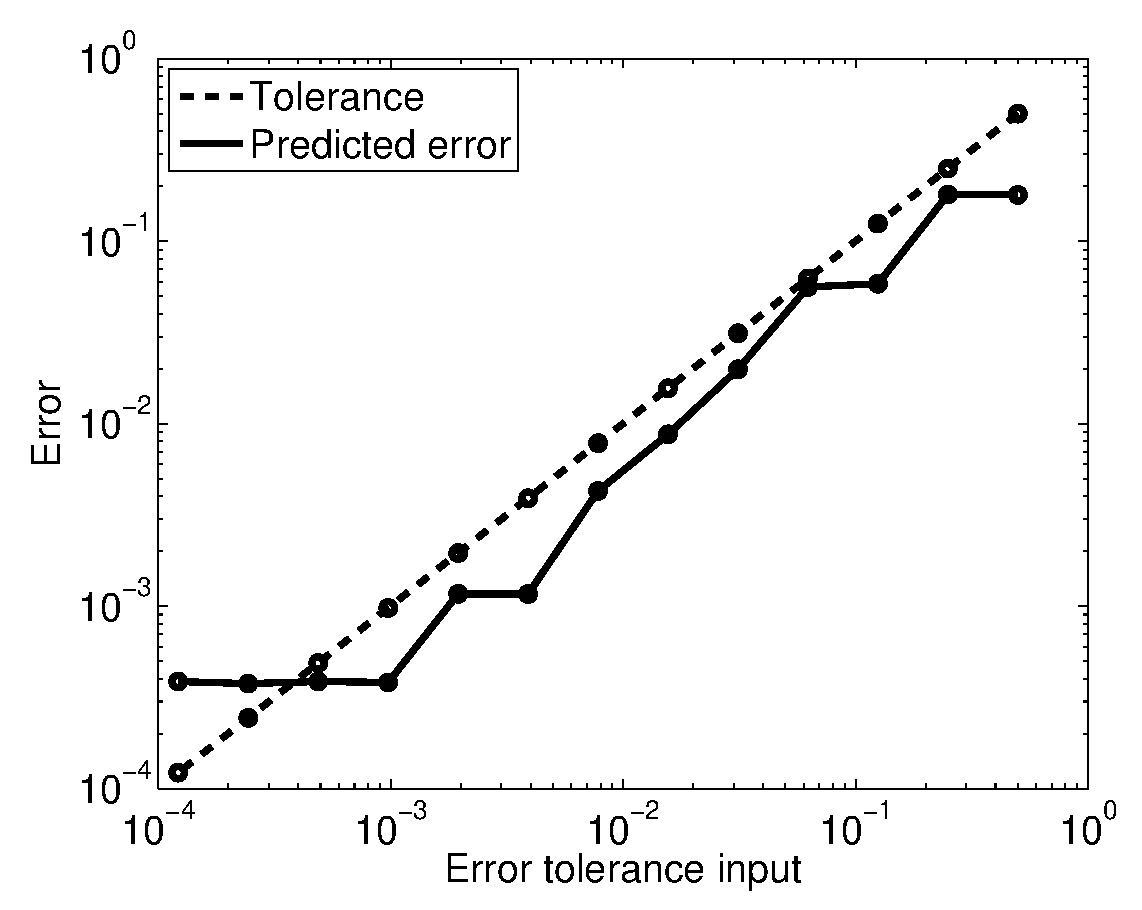
\includegraphics[width=5cm]{Images/Multicall_conv.eps} &
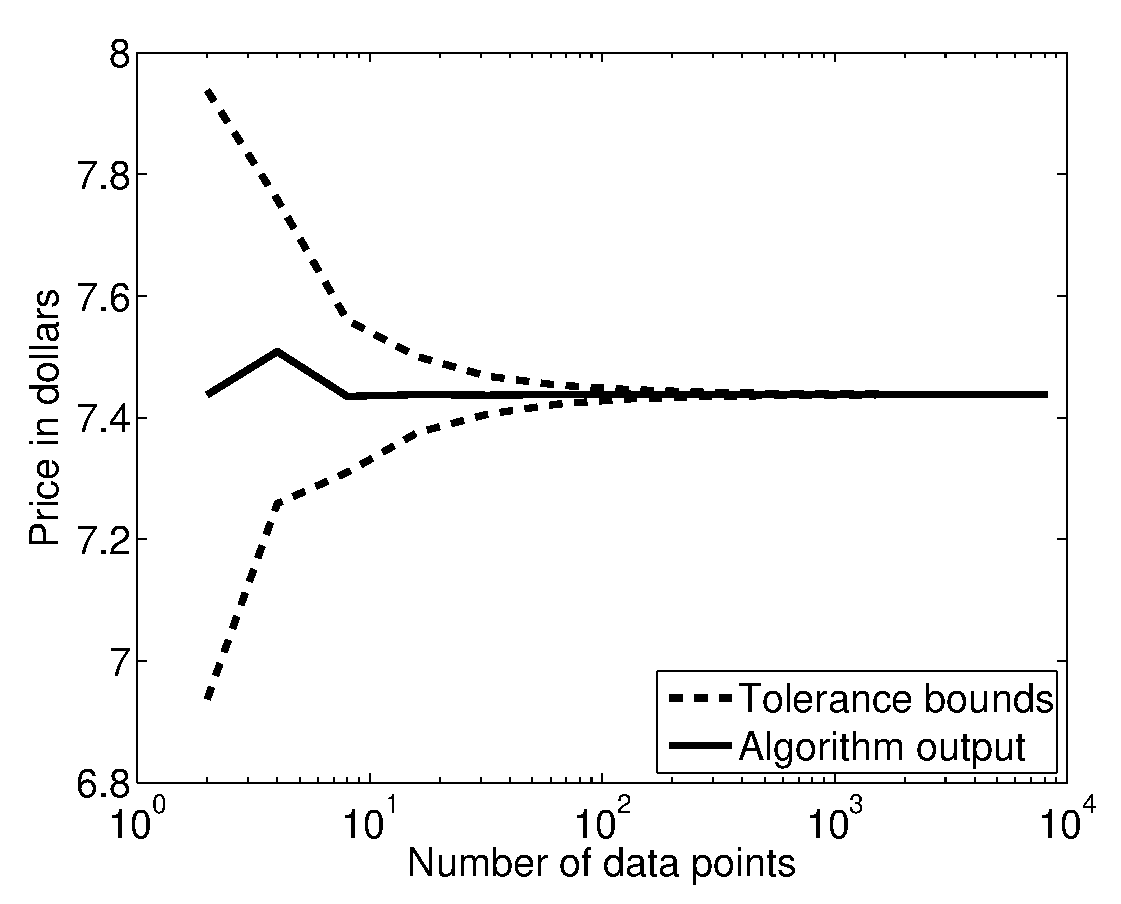
\includegraphics[width=5cm]{Images/Multicall_error.eps}\tabularnewline
a) & b)
\end{tabular}
\caption{a) Tolerance against predicted error, b) Price obtained with the tolerance bounds. \label{BasketOption}}
\end{figure}


\section{Discussion}
Fit the cones of functions into another well known space, rel error, discuss that is computed very fast....


\begin{acknowledgement}
Thanks to Dirk Nuyens, Pierre L'Ecuyer, Frances Kuo, NSF (Art Owen), Yizhi and Lan....
\end{acknowledgement}

\bibliographystyle{spmpsci.bst}
\bibliography{FJH22,FJHown22,lluisantoni}

\section*{Appendix A: Periodizing the Integrands}\label{periodizing}
For non periodic integrands $f$, we can use transformations $\phi$ to obtain periodic functions $g$ such that:
\begin{equation}\label{transeq}
\int_{\cube} f(\bsx)  \, \dif \bsx=\int_{\cube} g(\bst)  \, \dif \bst
\end{equation}
where
\begin{equation}\label{gdef}
g(t_1,\dots,t_d)=f(\phi(t_1),\dots,\phi(t_d))\phi'(t_1)\cdots\phi'(t_d)
\end{equation}

One example is the Baker's transform $\phi(t)=1-2\abs{t-0.5}$. A simple calculation in one dimension proves the equality \eqref{transeq} and by the Fubini theorem it can be extended to any dimension. Remark that this transform may generate a periodically extended $g$ not differentiable. Therefore, for smoother integrands $f$ we may loose differentiability after applying the transformation. However, really smooth transformations may introduce waviness. In any of both cases, it implies slower Fourier coefficients decay. See section \eqref{sumscoeff} for further implications on this paper.

Another option is described in \cite{SloJoe94}. Here, $\phi$ must be an increasing function which maps $[0,1]$ onto $[0,1]$. If $\phi'(0)=\phi'(1)=0$, by \eqref{gdef} function $g$ becomes periodic. The simplest polynomial fulfilling this conditions is $\phi(t)=3t^2-2t^3$. Again, as for the Baker's transform, this may produce a non differentiable $g$. One solution, if $f\in\cc^n$, is finding the polynomial requiring $\phi^{(i)}(0)=\phi^{(i)}(1)=0$  where $i=1,\dots,n+1$ for $f\in\cc^n$, implying $g\in\cc^n$. A part from polynomials, one could also consider the transform proposed by Sidi in \cite{Sid93}: $\phi(t)=t-\sin(2\pi t)/(2\pi)$.

\end{document}